\documentclass{standalone}

\begin{document}

\section[CHIMeRA analyses]{CHIMeRA analyses}\label{chimera:res}

The large amount of information provided by \textsf{CHIMeRA} network has to be analyzed to prove its efficiency.
A preliminary analysis was performed evaluating the nodes degree centrality (the number of links associated to each node).
The degree centrality is the simpler measure to quantify the importance of a node into a network: since our network-of-networks structure includes multiple node types we monitored it for each of them\footnote{
  We have chosen the degree centrality rather than other standard measures due to its numerical-simplicity/informative ratio.
  \textsf{CHIMeRA} network-of-networks includes a large amount of nodes, so the algorithmic complexity drastically affects the time performance.
  Degree centrality is given by summing the in- out-connections and thus it is the faster solution also with large matrix as in our case.
}.
In this way we can perform a preliminary overview of the full set of information in the network.
The results obtained by this test on degree centrality are shown in Tab.~\ref{tab:chimera_degree}.

\begin{table}
\centering
\begin{tabular}{lccccccc}
\hline\rowcolor{darkgrayrow}
                        & mean            &  std    &  min & 25\% & 50\% & 75\% &   max  \\
global degree           & 121.44          &  784.86 &    1 &    1 &    2 &    7 & 108147 \\
disease                 &  18.54          &  109.25 &    0 &    0 &    1 &    3 &  22911 \\
drug                    &  93.59          &  737.60 &    0 &    0 &    0 &    0 &  17750 \\
food                    &   0.03          &    0.32 &    0 &    0 &    0 &    0 &     12 \\
gene                    &   1.96          &   38.81 &    0 &    0 &    0 &    0 &   5605 \\
metabolite              &   0.37          &  154.73 &    0 &    0 &    0 &    0 &  85236 \\
phenotype               &   5.50          &  100.09 &    0 &    0 &    0 &    0 &   9732 \\
SNP                     &   0.65          &   21.96 &    0 &    0 &    0 &    0 &   4866 \\
metabolic pathway       &   0.09          &    2.81 &    0 &    0 &    0 &    0 &    594 \\
disease pathway         &   0.05          &    1.27 &    0 &    0 &    0 &    0 &    283 \\
drug-action pathway     &   0.14          &    6.79 &    0 &    0 &    0 &    0 &   1006 \\
drug-metabolism pathway &$6\times10^{-3}$ &    0.28 &    0 &    0 &    0 &    0 &     60 \\
signaling pathway       &$4\times10^{-3}$ &    0.29 &    0 &    0 &    0 &    0 &     49 \\
physiological pathway   &$1\times10^{-3}$ &    0.07 &    0 &    0 &    0 &    0 &     13 \\
macro pathway           &   0.48          &  106.06 &    0 &    0 &    0 &    1 &  59993 \\
\hline\\
\end{tabular}
\caption{Statistics of degree connections related to each node type stored in the \textsf{CHIMeRA} database.
For each node type the average, standard deviation, minimum value, maximum value and percentiles of the degree distribution are reported.
The first row shows the aggregated value of degree scores.
}
\label{tab:chimera_degree}
\end{table}

For each node type we computed the average number of connections and the most important parameters of each distribution (minimum, maximum, average, standard deviations and percentiles).
This preliminary analysis confirms what we have already discussed during the creation of the \textsf{CHIMeRA} structure and thus that the minimum number of connections is just $1$ (ref. min row in Tab~\ref{tab:chimera_degree}): disease nodes are the core of our network-of-networks model but they do not have a direct link with food nodes; at the same time, drug nodes, which are connected to the several other types do not include all of them.
Using the finer grain distinction between the metabolite-pathways (obtained by the information provided by HMDB) we noticed that the major part of their connections concern the \emph{macro pathway} category as expected: \emph{macro pathway}s identify the more general category in our nomenclature, including biological processes like \textsf{apoptosis}, \textsf{DNA replication fork} and \textsf{phosphatidylethanolamine biosynthesis}.
A better visualization of the network structure could be done counting the average number of connections between each node group, i.e the block matrix visualization of the underlying bipartite-graphs.
In Fig.~\ref{fig:chimera_bipartite} is shown this block matrix representation.

\begin{figure}[htbp]
\centering
\def\svgwidth{\textwidth}
\input{./img/chimera_net_mat.pdf_tex}
\caption{Block matrix representation of the \textsf{CHIMeRA} network.
We computed the average number of connections between each node group and the bipartite-graphs structure is highlighted.
}
\label{fig:chimera_bipartite}
\end{figure}

In Fig.~\ref{fig:chimera_bipartite} we can better appreciate the connections between the available information, visualizing and quantifying them.
As expected, the only node type which is connected to all the others is the \emph{disease} one: the only exception is given by \emph{food} nodes for the previously discussed reasons.
Our network-of-networks structure is very sparse and we do not have direct information of the major part of combinations (null blocks).
The only two node types which show a reasonably good interaction with other blocks are the \emph{disease} and \emph{drug} ones\footnote{
  For sake of clarity we have to highlight also the two diagonal blocks in our matrix, given by these two node types.
  They arise from the synonyms and related causes in the first case (information provided by synonym dictionaries and RXList), while in the second case they highlight the synergies or not (information given by DrugBank).
  A network adjacency matrix tends to nullify diagonal information and node self-loops to prevent numerical issues and to increase the amount of mathematical theorems for its analysis.
  We would stress that the showed matrix is not the adjacency matrix of \textsf{CHIMeRA} network but it is an aggregate representation of it.
  Thus, in our network each node has connections only with other nodes and no self-loops are present.
}.

The sparsity of \textsf{CHIMeRA} network-of-networks highlights all the pros and cons of our work.
More a matrix is sparse and more its management could be efficient from a numerical point-of-view: we are able to use a wide range of algorithms developed and tuned by sparse algebra; also the memory occupation could be optimized and it is a crucial task when we work with such a big quantity of data.
At the same time, it highlights the potentiality of our work: each block connection derives from a single database evaluation (in first approximation), and we can reasonably assume that each block represents a possible output of a query performed on that database.
In our global database we have the union of all these information and using at least the 2nd neighbors of a node (the nearest neighbors of each nearest neighbor of a node) we could obtain a mapping of all available information about it.
Moving along the matrix blocks, in fact, we can start from a gene and see only the associated diseases, which is comparable to a single-database query; since each disease is connected to all the other node types, the 2nd neighbors of our gene give a panoramic overview of all the biomedical agents associated to it.
This process is equivalent to an inference of missing blocks: if a gene is connected only to disease types, since all the other blocks are null, we can infer missing blocks using the links provided by disease nodes.
This is the real power of a such network-of-networks structure.
We would stress that the inference procedure could lead to incorrect biological associations, since it represents only an hypothesis unbacked up by data.
However, using more database sources we can easily integrate missing information using the developed processing pipeline and, thus, increase the reliability of our hypothesis.

To further investigate the information provided by our network using the computed degree scores, we evaluated degree distributions of each node type.
In Fig.~\ref{fig:chimera_degree} we show the degree distributions obtained considering the different node types individually.

\begin{figure}[htbp]
\centering
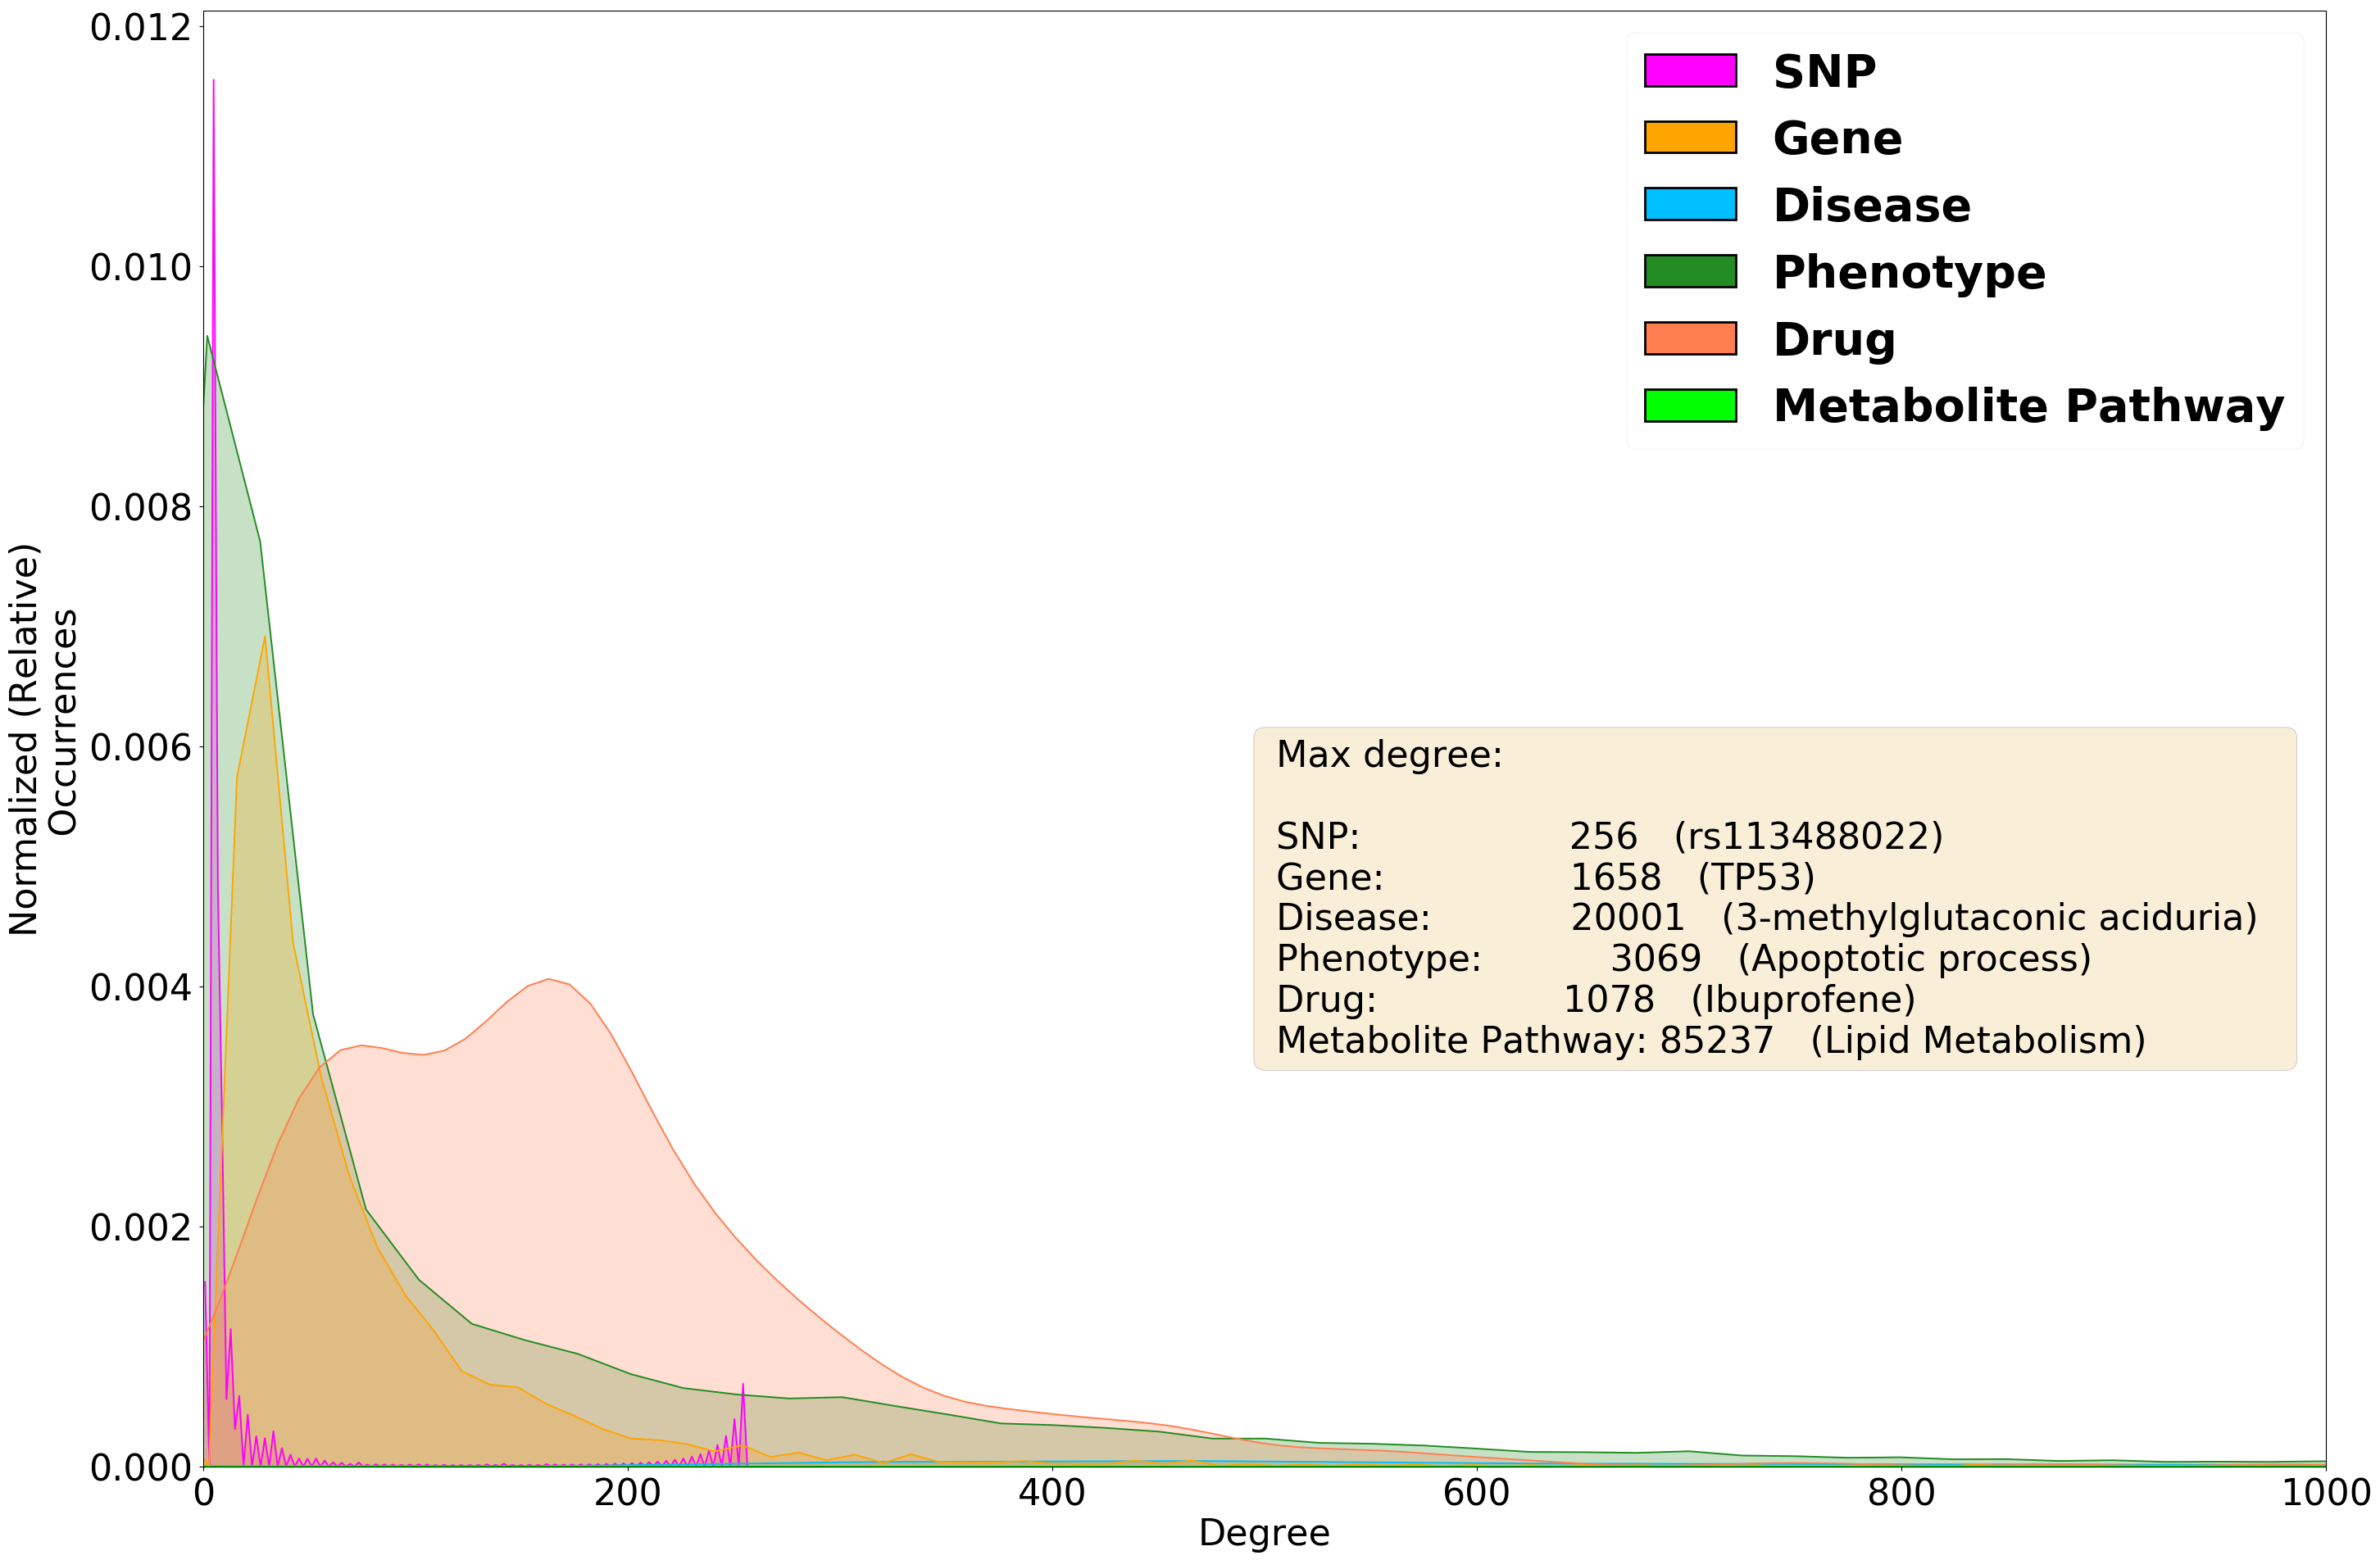
\includegraphics[width=.8\linewidth]{degree.png}
\caption{\textsf{CHIMeRA} degree distributions for different node types.
The plot is cut for visualization purposes.
The maximum degree node information are highlighted in the box.
}
\label{fig:chimera_degree}
\end{figure}

All the distributions showed in Fig.~\ref{fig:chimera_degree} have long tails, but we cut them for visualization purposes.
As expected and already highlighted by the previous analyses, the major part of node types have a not negligible amount of nodes with very low connectivity.
Many node types have also isolated elements, i.e nodes with $0$ degree.
This behavior could be due to two possible causes: 1) our pipeline tends to remove some information and, thus, some true positive associations; 2) there are some missing information in the original databases that could not be overcome by our merging.
Since the most part of isolated nodes are given by \emph{metabolites} (ref. Fig.~\ref{fig:chimera} in which the green dots around the plot are isolated metabolite nodes) we checked into HMDB the origin of these issues.
In a not negligible number of cases, HMDB does not provide a disease association to a given metabolite and it proves our second hypothesis, preserving the efficiency of our pipeline.

A more interesting result is obtained considering the most central nodes, i.e the node related to the maximum degree score.
This information could be used also as validity check of the structure.
As in the \textsf{SymptomsNet} case (ref. \ref{chimera:symptomsnet}), we expect a reasonable interpretation of the most central nodes.
These results are shown in the yellow box of Fig.~\ref{fig:chimera_degree}.

The most central node for the SNP node type is \href{https://www.ncbi.nlm.nih.gov/snp/rs113488022}{\textsf{rs113488022}}, well known polymorphism, validated by more than 70 public researches.
This SNP is related to a wide range of cancer diseases and its clinical significance has been proved in different studies.
It is always hard to discuss about the more or less importance of a SNP compared to the others, but its relation to several cancer types confirms its centrality score in our network structure.
A more easily interpretable result is given by the most central gene, the \href{https://ghr.nlm.nih.gov/gene/TP53}{\textsf{TP53}}.
\textsf{TP53} is a crucial gene in many tumor diseases and its importance is well mirrored in our network structure.
The major part of diseases inserted into public databases are related to tumor researches, and thus it was quite obvious to obtain n high centrality of this gene in our network.
For the same reasons also the most central node for the \emph{phenotype} type should be a tumor related characteristic: as expected, the most central node in this case is given by the \textsf{apoptotic process}, i.e the process which regulates the programmed cell death, which is largely involved in tumor diseases.

As previously discussed about \emph{disease} and \emph{drug} types, we have to consider a large set of available connections for them.
Thus, we expected that a central node in these cases would be given by a quite generic entry.
About \emph{disease} type, in fact, we found as most central node the \href{https://en.wikipedia.org/wiki/3-Methylglutaconic_aciduria}{\textsf{3-methylglutaconic aciduria}}, a congenital metabolism anomaly related to leukemia.
Despite this disease could be considered quite rare, its importance in our network structure is certainly given by the large amount of metabolite connections (we remember that HMDB provides a very large amount of \emph{metabolite} nodes that overcome the number of all the other node types, except by SNPs).
The large quantity of metabolites in our structure weights on the number of disease connections and it proves the high centrality of a metabolic disease despite a genetic one.
Moreover, we have also to take into account that this disease is related to leukemia, so we would have also a large set of genes and SNPs associated to it.

Considering the \emph{drug} type, we obtained a very common drug as expected, given by the \href{https://en.wikipedia.org/wiki/Ibuprofen}{\emph{Ibuprofene}}.
\emph{Ibuprofene} is a very common anti-inflammatory drug that is used for treating pain, fever and inflammation which are all very general symptoms associated to a wide range of possible diseases.
Thus, it is reasonable to assume that its number of connections is greater than other (more target specific) drugs.

A more in-depth explanation must be provided for the \emph{metabolite pathway} type, where there are no seemingly reasonable explanations that prefer the found \textsf{lipid metabolism} to other macro-metabolite pathways.
To explain its centrality we, once more time, come back to the original databases and to HMDB in this case.
From a thorough inspection of HMDB we noticed that the most of them were studied using NMR chemical shift procedure.
NMR chemical shift is a very common spectroscopy procedure to analyze biological compounds, but its signal is hardly related to particular nucleus types (e.g $^1H$, $^{13}C$, $^{15}N$, $\cdots$).
We could broadly describe this technique saying that as much hydrogen-like or carbonic-like structures are into the biological sample and much the signal should be easy to analyze.
The metabolite relation to lipid metabolism is thus easy to study than other metabolism kinds, due to the large quantity of resonant nuclei involved\footnote{
  Fatty acids in lipid mixtures are widely studied using NMR chemical shift since their molecular structure involves multiple resonant nuclei such $^{13}$C, $^{31}$P and $^1$H.
}.
This proves the high centrality of \textsf{lipid metabolism} regard other metabolite pathways.

These results are only preliminary analyses of \textsf{CHIMeRA} network-of-networks structure, but they are already able to clarify some potential use of our work.
The only things that remain to be discussed are the usability and release of this new database to the research community.


\end{document}
